\documentclass[12pt]{article}

\usepackage[dvips,letterpaper,margin=0.75in,bottom=0.5in]{geometry}
\usepackage{cite}
\usepackage{slashed}
\usepackage{graphicx}
\usepackage{amsmath}

\usepackage[T1]{fontenc}
\usepackage[ttdefault=true]{AnonymousPro}
\usepackage{fancyvrb}

\begin{document}


\title{Arduino Digital Scope} 

\maketitle

\section{Introduction}

In this lab, you will construct a single-channel digital oscilloscope using the analog-to-digital converter (ADC) on the Arduino Uno.  Your oscilloscope will not compete with LeCroy or Tektronix just yet, but for \$30 it will cover the entire audio range.  Not bad!

\section{Free-Running ADC Mode}

An initial sketch {\tt Scope} is provided with this lab to get you started.  To achieve the fastest possible sample rate, your scope will operate the ADC in free-running mode.  In this mode, the ADC continuously samples the input, and the new sample is processed immediately after it becomes available.

The primary way that processors handle time critical operations is through interrupts.  An interrupt is a hardware signal sent to the processor indicating that an event has occurred.  The code the processor is currently running is temporarily halted and instead specialized code contained in an interrupt service routine programmed to handle that particular event is executed.   When the interrupt service routine exits, the processors returns to executing the code that was running before the interrupt.   Generally, one wants the interrupt service routine to be as lightweight as possible, handling only the time critical task.

In this case, we first use driver commands to configure the hardware to run the ADC continuously and send the appropriate interrupt, then we provide an interrupt service routine to process the new sample.
The driver commands to set the ADC to sample analog pin 0 in free running mode on the Uno are already included in the ``Scope" sketch:
 \begin{verbatim}
  ADCSRA = 0;             // clear ADCSRA register
  ADCSRB = 0;             // clear ADCSRB register
  ADMUX |= (adc & 0x07);    // set A0 analog input pin
  ADMUX |= (1 << REFS0);  // set reference voltage
  ADMUX |= (1 << ADLAR);  // left align ADC value to 8 bits from ADCH register
  // sampling rate is [ADC clock] / [prescaler] / [conversion clock cycles]
  // for Arduino Uno ADC clock is 16 MHz and a conversion takes 13 clock cycles
  ADCSRA |= (1 << ADPS2);                     // 16 prescaler for 76.9 KHz
  ADCSRA |= (1 << ADATE); // enable auto trigger
  ADCSRA |= (1 << ADIE);  // enable interrupts when measurement complete
  ADCSRA |= (1 << ADEN);  // enable ADC
  ADCSRA |= (1 << ADSC);  // start ADC measurements
\end{verbatim}
Where $\rm adc=0$ specified elsewhere sets the ADC channel to A0.  The interrupt service routine which handles each new sample is also provided:
\begin{verbatim}
  ISR(ADC_vect){
    if (isamp < max_samples){
      buf[isamp++]=ADCH;
    }
  }    
\end{verbatim}
This code is executed every time the hardware has completed a new sample, and it simply copies the sample into the next place in a buffer.  This initial version of your scope has no trigger. When the buffer is full, it simply dumps the first 500 samples to the serial output, which can then be plotted using the Serial Plotter provided by the Arduino IDE.  The serial plotter has a fixed width of 500 entries, so by sending exactly 500 samples, we display one captured wave form at a time.

\section{Using the Scope Sketch}

{\bf We won't be building an analog front-end for this digital scope, so you'll need to be careful not to damage the ADC by driving it outside of the $0$ to $5~\rm{V}$ range!} \\ 

\noindent
{\bf Step 1:}  Make certain the your function generator is set to ``high impedance output" under setup and set it to deliver a $1~\rm kHz$ sine wave with high value of $5~\rm V$ and a low value of $0~\rm V$.  Double check that you have the settings correct before connecting it!  In particular, you want to make sure your a sending an {\bf offset} sine wave, which ranges from $0$ to $5~\rm V$, and not, e.g., one from $-2.5~\rm V$ to $2.5~\rm V$!   Once your function generator is setup properly (and confirmed!) configure your Uno with the Scope sketch.  Connect the ground of your function generator to ground on your Arduino, and connect the signal to analog pin 0.\\

\noindent
{\bf Step 2:}  Open the serial plotter tool.  The serial plotter simply plots the most recent 500 lines received on the serial port.  The Scope sketch initializes the serial port with a baud rate of 115200, so you'll need to set the serial plotter baud rate to the same value. \\

\begin{figure}[htbp]
\begin{center}
{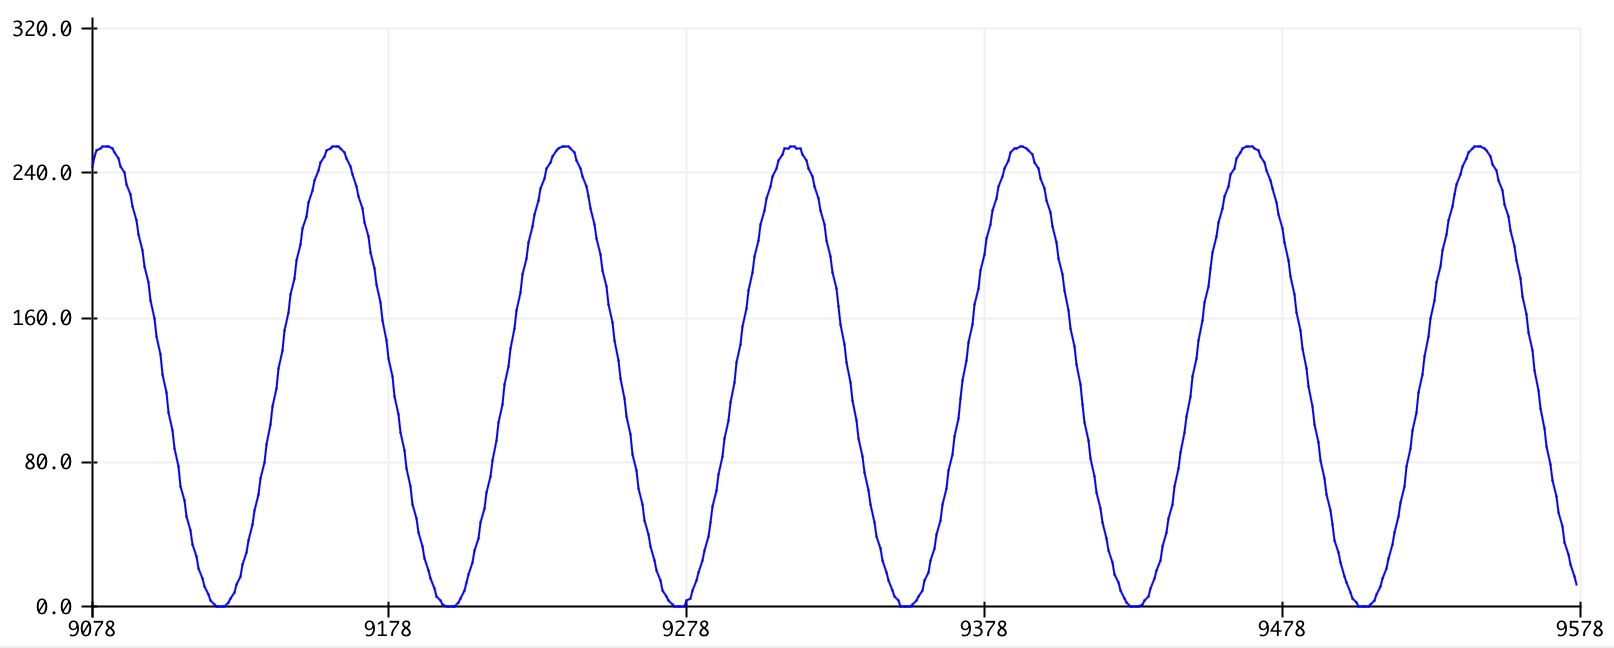
\includegraphics[width=0.75\textwidth]{figs/tracea.png}}
{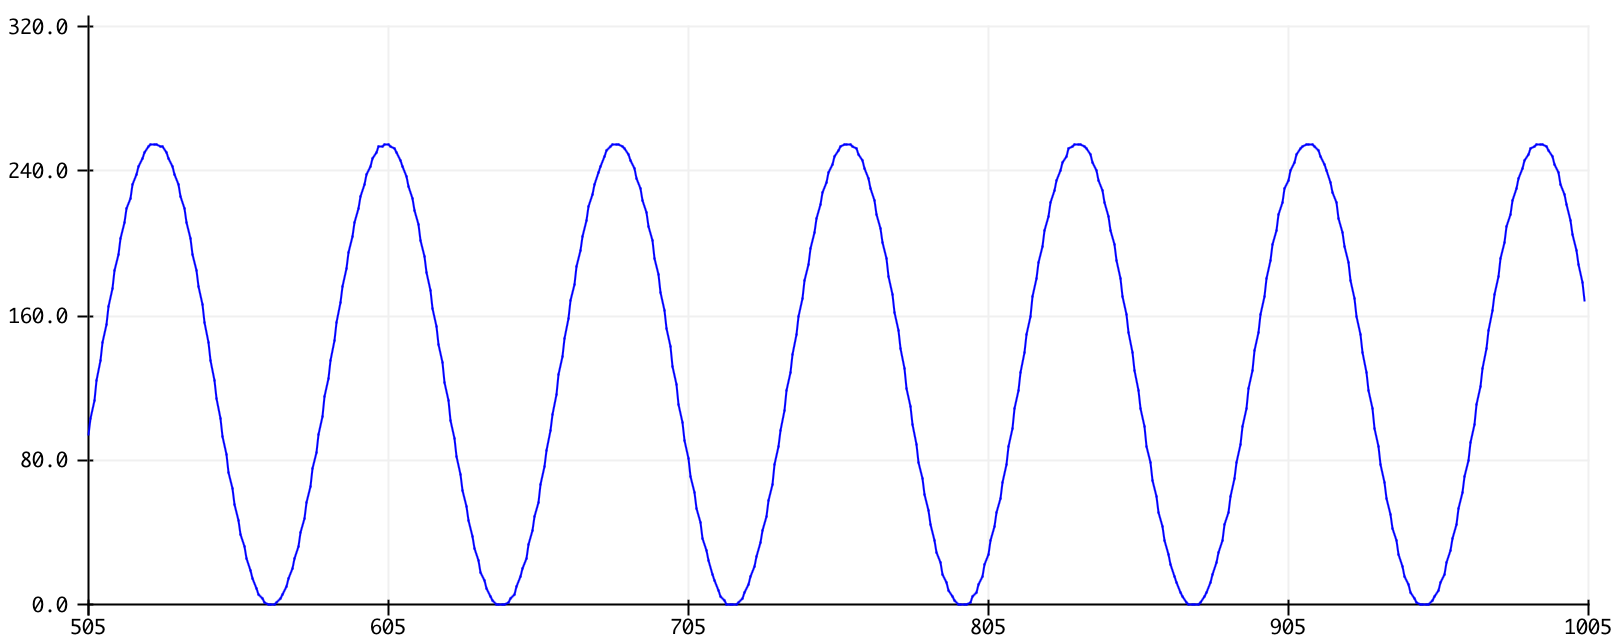
\includegraphics[width=0.75\textwidth]{figs/traceb.png}}
\end{center}
\caption{\label{fig:traces} two example wave forms captured from the {\rm scope}  sketch.  Note that the phase of the waveform varies from sample to sample, due to the lack of trigger.}
\end{figure}

You should observe sine waves like those in Fig.~\ref{fig:traces} in the serial plotter tool.  Note that the phase changes from one waveform to the next, because this sketch has no trigger requirement, it is simply displaying the waveform at a random time.

\section{Digital Trigger}

Your first task is to add a trigger requirement to the display of the waveform.  You trigger should have a few adjustable parameters as follows:
\begin{itemize}
 \item {\bf threshold}:  trigger just at the point when waveform goes above this threshold
 \item {\bf offset}:  you should display an adjustable number of samples before the trigger
\end{itemize}

The serial plotter is convenient, but a bit clunky.  Keep in mind that it displays the most recent 500 lines, so you'll always want to output your waveform as exactly 500 samples written on 500 lines.

For the first iteration, you should simply check if and where the trigger condition is met in the buffer, once it is complete.  Do not try to keep up with the interrupt routine in the loop!  Instead, wait until the buffer is full, then check for a trigger.  You should only trigger if the condition occurs where there are enough samples available before the trigger to provide the specified offset, and enough samples available after to provide a complete waveform (500 samples wide, including offset).

Once your trigger is working, you should see that the output is always at the same phase, and that you can adjust this phase with the offset parameter.  If you {\em carefully} adjust the voltage from the function generator so that it stays below your threshold, you should no longer trigger.

Once the normal trigger mode is working, see if you can implement an automatic trigger mode.  This will output the normal triggered output if available, otherwise, it will simply output the waveform from a randomly chosen time (such as the start of the buffer, as in the initial version.)

\section{A Deadtime-less Design}

The design above, where we capture samples as fast as possible until the buffer is full, and then examine the buffer contents at our leisure, is an efficient design, particularly when the available CPU speed is limited, and often this is the best we can do, particularly if the digital signal processing stage is quite extensive.  It comes with a serious drawback, however!  While the full buffer is being processed, the incoming waveform is ignored.  This is no problem for periodic functions like the sine wave, but if we are using this scope to say, trigger on a cosmic ray muon, this so-called {\em deadtime} is a serious drawback!

Fortunately, checking for our trigger condition is not too computationally extensive, if we are careful about it!  In this mode of running, the interrupt service routine for the ADC should start as something like this:
\begin{verbatim}
  ISR(ADC_vect){
     buf[isamp++]=ADCH;
     if (isamp == max_samples){
       isamp = 0;
     }  
  }
\end{verbatim}
This turns the buffer into a {\em circular buffer}.  When it is full, it simply begins writing again at the bottom.

Your task now is to add a trigger requirement to the circular buffer in a way that does not incur any dead time.  Here's why this is a serious challenge.  You might first be tempted to simply check the contents of the circular buffer from within the loop function, to avoid interfering with the time critical sample collection.  This is a healthy impulse to keep the ISR routine as simple as possible, and a solid design, except that you will likely find that the loop falls behind the interrupt driven sample collection.  However, if on the other hand, you load down your ISR too heavily with additional trigger requirements, your sample rate slows down and becomes jittery:  an unacceptable outcome for a scope with our name on it!  What worked for me was to put a carefully chosen subset of small, time critical operations into the ISR, and leave as much as possible to the loop.

In my design, I extended the above ISR to do the following:
\begin{itemize}
\item {\tt boolean buffered}:  whenever the roll-over of isamp occurs, {\tt buffered} is set to true.   This flag tells me if the circular buffer has filled at least once, which ensures that my offset for the trigger is covered.
I leave resetting this to false (for the next trigger acquisition) to the loop routine!
\item {\tt boolean current}:  I check if the current sample is above threshold, for example:
\begin{verbatim}
  boolean current  = buf[isamp] > 128;
\end{verbatim} 
\item {\tt boolean trigger}: my trigger condition is  {\tt buffered \& previous \& current}.  If this condition is not met, I set previous=!current for the next interrupt.
\item {\tt int count:}  if the trigger flag is true, I increment the count.  When the count reaches the required number of post trigger samples, the ISR stops filling the buffer to allow for readout.  (Post-trigger readout dead time is acceptable for our purposes.)  The resetting of count for the next trigger is handled in the loop after reading out.
\end{itemize} 
Readout and then resetting of the flags for the next trigger is all handled in the loop, once the post-trigger {\tt count} reaches the desired number of post-trigger samples.  This design worked well for me, but there are certainly other ways.  See what you can do!

\section{Bandwidth Limitations}

When the frequency of your input signal exceeds the frequency of your sampling rate, you will begin to see aliasing such as in Fig.~\ref{fig:aliasing}.  Increase the frequency of your input function and observe the onset of aliasing.  What is the approximate bandwidth of your scope? 
\begin{figure}[htbp]
\begin{center}
{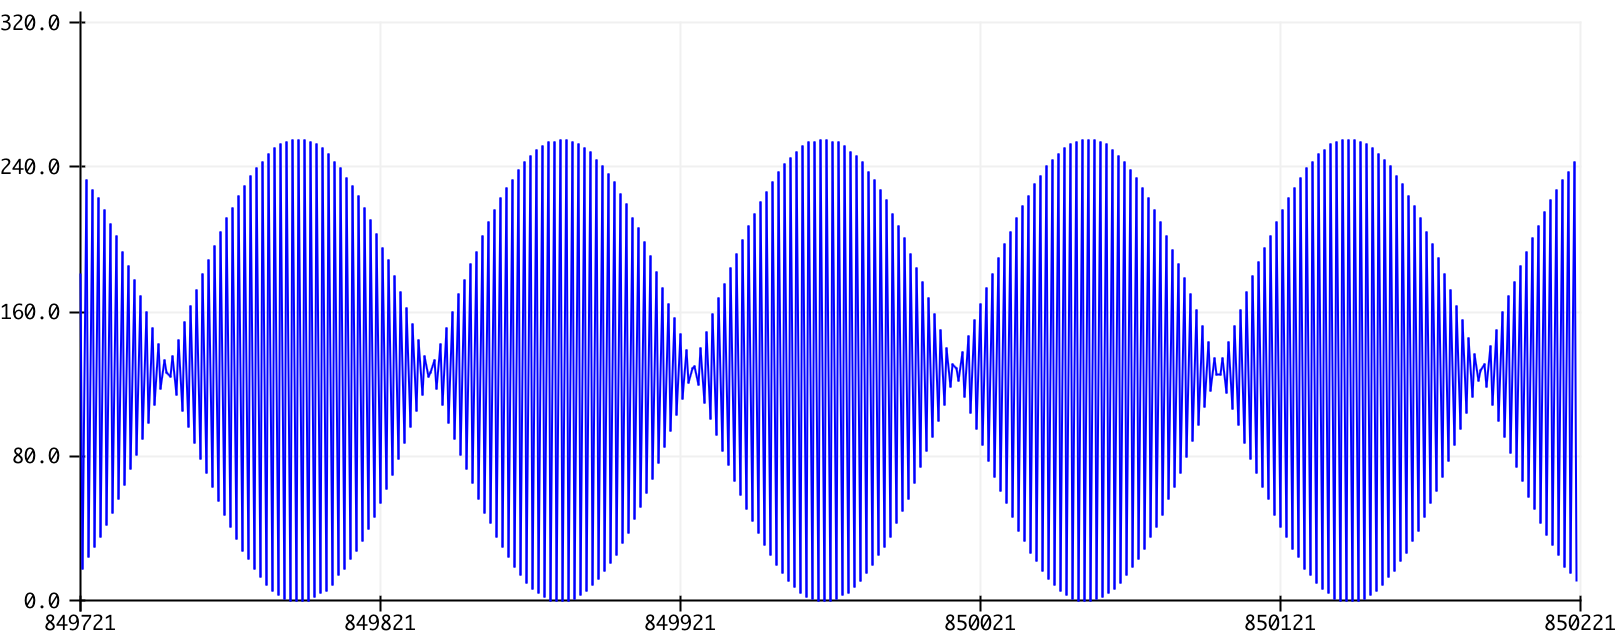
\includegraphics[width=0.75\textwidth]{figs/aliasing.png}}
\end{center}
\caption{\label{fig:aliasing} Aliasing of a high-frequency input.}
\end{figure}


\end{document}
